\chapter{System Design}
\thispagestyle{plain}
\label{System Design}


\section{Architecture Overview}

The architecture of the system comprises of several modules that process a given input log file. After going through the several components we give out a RDF (Resource Description Framework) file as output. The modular nature of the architecture allows us to add more specialists to the existing framework. Thus, the framework was designed keeping scalability in mind. Figure~\ref{fig:system_architecture} shows the block diagram of the system architecture. It begins with \textit{Tabulate} module, where the input log file is parsed to detect its structure. Once the structure is detected the structured log file is separated into columns. These columns are they passed to the \textit{Decode} stage. In the \textit{Decode} module the columns are checked against various classifiers to find a match. After checking against different classifiers, the columns are given a score against every classifier in the system. The scores form a ranked list of probable classes for the columns in the log file. This ranked list is used in the \textit{Relationship Generator} to identify the relations between various columns in the log file. Once the columns are identified and the relationships have been detected, the \textit{Generate RDF} module will produce a set of RDF triples to represent the inferred semantics. The four major modules have been described in detail in rest of the section.


\begin{figure}[h]
	\centering
	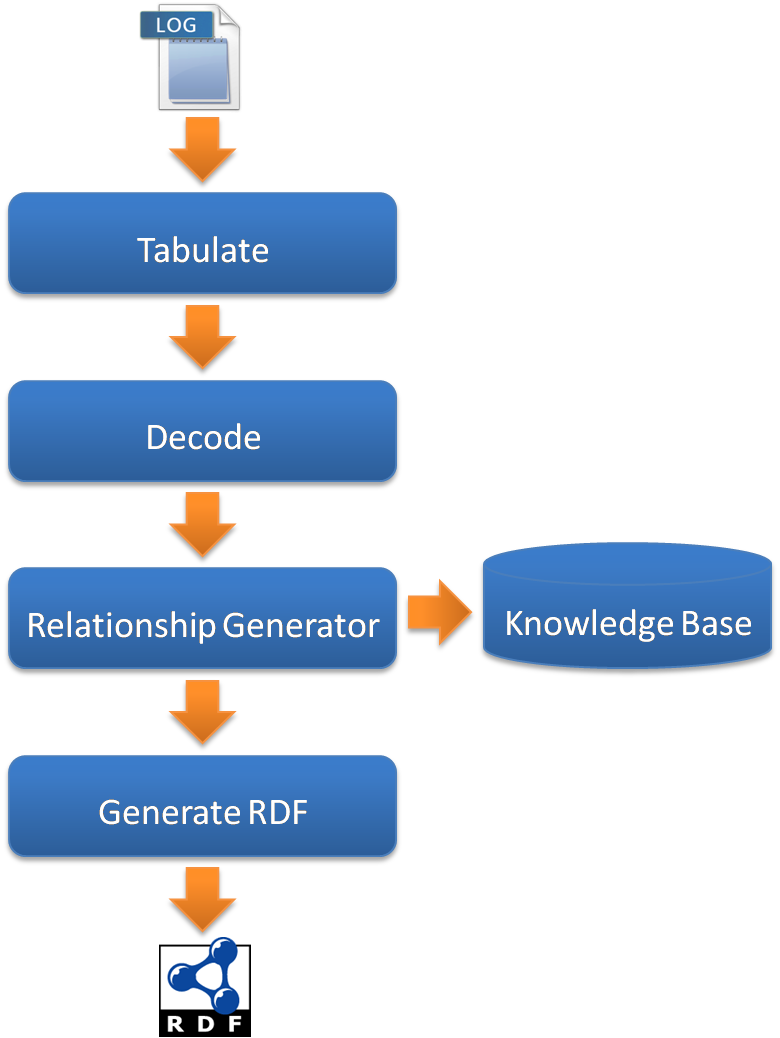
\includegraphics[width=\textwidth, height=0.5\textheight, keepaspectratio] {system_architecture.png}
	\caption{System Architecture}
	\label{fig:system_architecture}
\end{figure}


\subsection{Tabulate}
\label{Tabulate}

The \textit{Tabulate} module takes the structured log file as input and gives out a possible set of columns to the \textit{Decode} module for classification. The input log file can have any structure and the module will try to detect columns in it. The log file undergoes multiple iterations for the following reasons:
\begin{itemize}
\item To split the log file based on delimiters
\item To detect consistent number of columns throughout the log file
\item To detect and separate sub-columns
\end{itemize}

In the first iteration of the \textit{Tabulate} module, we split the log files using generic delimiters like space, square braces, round braces, single and double quotes. For braces and quotes we consider only those that are in pairs. Every row is thus separated in varied number of columns that may or may not be consistent. 

Although most of the lines in a structured log file have fixed number of columns, it is not necessary that after separating on the above delimiters we will get equal number of columns. Also, some log entries can be outliers due to consistency in the way the logs are generated. But in most of the cases, there is a textual description at the end of the log entry which does not have a fixed number of words. If the description is not enclosed in a brace or quote, then it will be divided into several different columns. Considering this fact, we dynamically decide the number of columns that are to be extracted. For this, we put a threshold on the percentage of rows that will be considered in the system. We select rows starting with the ones that have the highest number of columns. We then select the next set of rows that have the second highest number of columns. We continue this process till we reach the threshold number of rows. At this moment we record the number of columns of the current set of rows. This is the number of columns that we choose to output from the system. All the rows having columns less than the selected number of columns are discarded. We keep the threshold pretty high (above 70 \%), so as to collect more number of rows. We also tried keeping the rows that have columns less than the selected number of columns and utilize them in the \textit{Decode} module. It was observed if a large percent of log entries have consistent columns, then the remaining smaller percent usually forms abnormal entries. Thus they create noise in the \textit{Decode} module when trying to detect the class of the column.

In the third iteration, we loop through the columns that are already separated in the previous iterations. In this iteration, we check the columns to detect sub-columns. We use the same set of delimiters to split the columns further. If all the elements in a particular columns are separable, then we split the column into multiple sub-columns. Before separation, we run that complete column through the \textit{Decode} module to check if the whole column matches any of the known classes. If there is a match found, then there is no need of splitting the column, as we can use the column as a whole.


\subsection{Decode}
\label{Decode}

The \textit{Decode} module does the work of assigning classes to the columns given by the \textit{Tabulate} module. For the classification of columns we created an extension of the specialists approach implemented by Puranik~\cite{puranik2012specialist}. Puranik defines a specialist as ``an entity that has expertise in the domain for which it is a specialist''. The mentioned specialists system was created for generic table data found on the Internet like SSN, phone numbers, addresses, etc. We extend this system to classify specific fields that are usually found in log files viz., timestamps, IP addresses, URLs, etc.

Every column is passed through the specialists in the system. All the specialists give their score to the column based on how well the column matches the class of the specialist. We normalize this score to form a ranked list to predict the class of the system. If there is no match to any of the specialists then the columns is classified as `NA' (No Annotation). The normalized scores can also be considered as the confidence with which the specialists classifies a particular column into its respective class.

Specialists can be of different types like regular expression based specialists, dictionary based specialists and classifier based specialists. Currently we are using only regular expression based and dictionary based specialists. But we can further extend it to use classifier based specialists as well. Following is the list of specialists present in the current system:

\begin{enumerate}
\item \textbf{Timestamp Specialist}\\
The Timestamp specialist is a regular expression based specialist, which handles a lot of timestamp formats which are used in various systems for logging. This could also be implemented as a classifier based specialist using the Date specialist implemented by Puranik~\cite{puranik2012specialist}.
\item \textbf{IP Address Specialist}\\
The IP Address specialist is a regular expression based specialist. It checks for valid IP address formats and also makes sure that they are in a valid range.
\item \textbf{URL Specialist}\\
The URL specialist is a regular expression based specialist, which looks for various URL formats viz., HTTP, HTTPS, FTP, FTPS. It also detects URL having basic authentication.
\item \textbf{Filepath Specialist}\\
The Filepath specialist is also a regular expression based specialist. It looks for filepaths irrespective of the underlying system.
\item \textbf{Email Specialist}\\
The Email specialist is a regular expression based specialist, that looks for valid email formats in the given column. This follows the Internet standards to detect a valid email.
\item \textbf{HTTP Status Code Specialist}\\
The HTTP Status Code specialist is dictionary based specialist. It looks for the HTTP status code values provided by the W3 standards. These HTTP status codes are integer values.
\item \textbf{HTTP Method Specialist}\\
The HTTP Method specialist is a dictionary based specialist. It looks for the known HTTP verbs / methods like GET, PUT, POST, DELETE, etc.
\item \textbf{HTTP Protocol Version Specialist}\\
The HTTP Protocol Version specialist is a dictionary based specialist, which looks for the known HTTP protocol versions. The HTTP protocol versions are in a string format.
\end{enumerate}

We can easily extend the system to add more specialist to detect other fields in the log files. These specialists can be regular expression based or dictionary based specialists. For instance, if a system administrator decides to have a specialist for server names, then they can have a dictionary based specialist. They will keep a dictionary with all the server names. In future, if the our system comes across a log file with server name as the column, it will detect and classify the column precisely.
 

\subsection{Relationship Generator}
\label{Relationship Generator}

\subsection{Generate RDF}
\label{Generate RDF}